% Digital Logic Report Template
% Created: 2020-01-10, John Miller

%==========================================================
%=========== Document Setup  ==============================

% Formatting defined by class file
\documentclass[11pt]{article}

% ---- Document formatting ----
\usepackage[margin=1in]{geometry}	% Narrower margins
\usepackage{booktabs}				% Nice formatting of tables
\usepackage{graphicx}				% Ability to include graphics

%\setlength\parindent{0pt}	% Do not indent first line of paragraphs 
\usepackage[parfill]{parskip}		% Line space b/w paragraphs
%	parfill option prevents last line of pgrph from being fully justified

% Parskip package adds too much space around titles, fix with this
\RequirePackage{titlesec}
\titlespacing\section{0pt}{8pt plus 4pt minus 2pt}{3pt plus 2pt minus 2pt}
\titlespacing\subsection{0pt}{4pt plus 4pt minus 2pt}{-2pt plus 2pt minus 2pt}
\titlespacing\subsubsection{0pt}{2pt plus 4pt minus 2pt}{-6pt plus 2pt minus 2pt}

% ---- Hyperlinks ----
\usepackage[colorlinks=true,urlcolor=blue]{hyperref}	% For URL's. Automatically links internal references.

% ---- Code listings ----
\usepackage{listings} 					% Nice code layout and inclusion
\usepackage[usenames,dvipsnames]{xcolor}	% Colors (needs to be defined before using colors)

% Define custom colors for listings
\definecolor{listinggray}{gray}{0.98}		% Listings background color
\definecolor{rulegray}{gray}{0.7}			% Listings rule/frame color

% Style for Verilog
\lstdefinestyle{Verilog}{
	language=Verilog,					% Verilog
	backgroundcolor=\color{listinggray},	% light gray background
	rulecolor=\color{blue}, 			% blue frame lines
	frame=tb,							% lines above & below
	linewidth=\columnwidth, 			% set line width
	basicstyle=\small\ttfamily,	% basic font style that is used for the code	
	breaklines=true, 					% allow breaking across columns/pages
	tabsize=3,							% set tab size
	commentstyle=\color{gray},	% comments in italic 
	stringstyle=\upshape,				% strings are printed in normal font
	showspaces=false,					% don't underscore spaces
}

% How to use: \Verilog[listing_options]{file}
\newcommand{\Verilog}[2][]{%
	\lstinputlisting[style=Verilog,#1]{#2}
}

\begin{document}

\title{ELC 2137 Lab 09: ALU with Input Register}
\author{My Nguyen}

\maketitle

\section*{Summary}
This lab's purpose is to get a better understanding SR latch, D latch, D flip-flip and D-register with combinational and regular sequential logic. First part is to create a register module that uses parameter to generate register module with different number of bit for input and output. Then, create a 8-bit ALU module using the provided code. Afterward, create top\_lab9 and import basys3.xdc with correct constraints as a top-level module to do on-board testing. Finally, import basys3\_lab9.sv file to do top-level simulation.

\section*{Expected results tables}
\begin{table*}[ht]\centering
	\caption{\textit{register} expected results table}
	\label{ALU:tbl:register_ERT}\medskip
	\begin{tabular}{l|rrrrrrrrrrr}
		Time (ns): & 0-5 & 5-10 & 10-15 & 15-20 & 20-25 & 25-30 & 30-35 & 35-40 & 40-45 & 45-50 & 50-55 \\
		\midrule
		D (hex) & 0 & 0 	  & A & A 	    & 3 	     & 3 	   & 0 	     & 0 & 0$\to$6 & 6 & 6 \\
		clk     & 0 & 1 	  & 0 & 1 	    & 0 	     & 1 	   & 0 	     & 1 & 0 	   & 1 & 0 \\
		en  	& 0 & 0 	  & 1 & 1	    & 1$\to$0 & 0$\to$1 & 1$\to$0 & 0 & 0$\to$1 & 1 & 1 \\
		rst 	& 0 & 0$\to$1 & 0 & 0 	    & 0 		 & 0 	   & 0		 & 0 & 0	   & 0 & 0 \\
		\midrule
		Q (hex) & X & X$\to$0 & 0 & 0$\to$A & A		 & A	   & A 		 & A & A$\to$6 & 6 & 6\\
		\bottomrule
	\end{tabular}
\end{table*}

\begin{table*}[ht]\centering
	\caption{\textit{alu} expected results table skeleton}
	\label{ALU:tbl:alu_ERT}\medskip
	\begin{tabular}{l|rrrrrr}
		Time (ns): & 0-10 & 10-20 & 20-30 & 30-40 & 40-50 & 50-60 \\
		\midrule
		in0 & A & A & A & A & A & A \\
		in1 & B & B & B & B & B & B \\
		op	& 0 & 1 & 2 & 3 & 4 & 5 \\
		\midrule
		out & 15 & FF & 0A & 0B & 01 & 0A \\
		\bottomrule
	\end{tabular}
\end{table*}


\section*{Simulation Waveform}
\begin{figure}[ht]
	\centering
	\includegraphics[width=\textwidth,trim=24cm 19cm 0.5cm 5.5cm,clip]{"regit"}
	\caption{Register ERT}
	\includegraphics[width=\textwidth,trim=24cm 23cm 0.5cm 5.5cm,clip]{"alu}
	\caption{ALU ERT}
	\includegraphics[width=\textwidth,trim=22cm 18.5cm 0.5cm 5.5cm,clip]{"sim"}
	\caption{Top-Level Simulation ERT}
\end{figure}


\section*{Pictures}
\begin{figure}[ht]
	\centering
	\includegraphics[width=12cm]{"board/step1"}
	\caption{Adding 0}
	\includegraphics[width=12cm]{"board/add"}
	\caption{Addition Operation}
\end{figure}
\begin{figure}[ht]
	\centering
	\includegraphics[width=12cm]{"board/sub"}
	\caption{Subtraction Operation}
	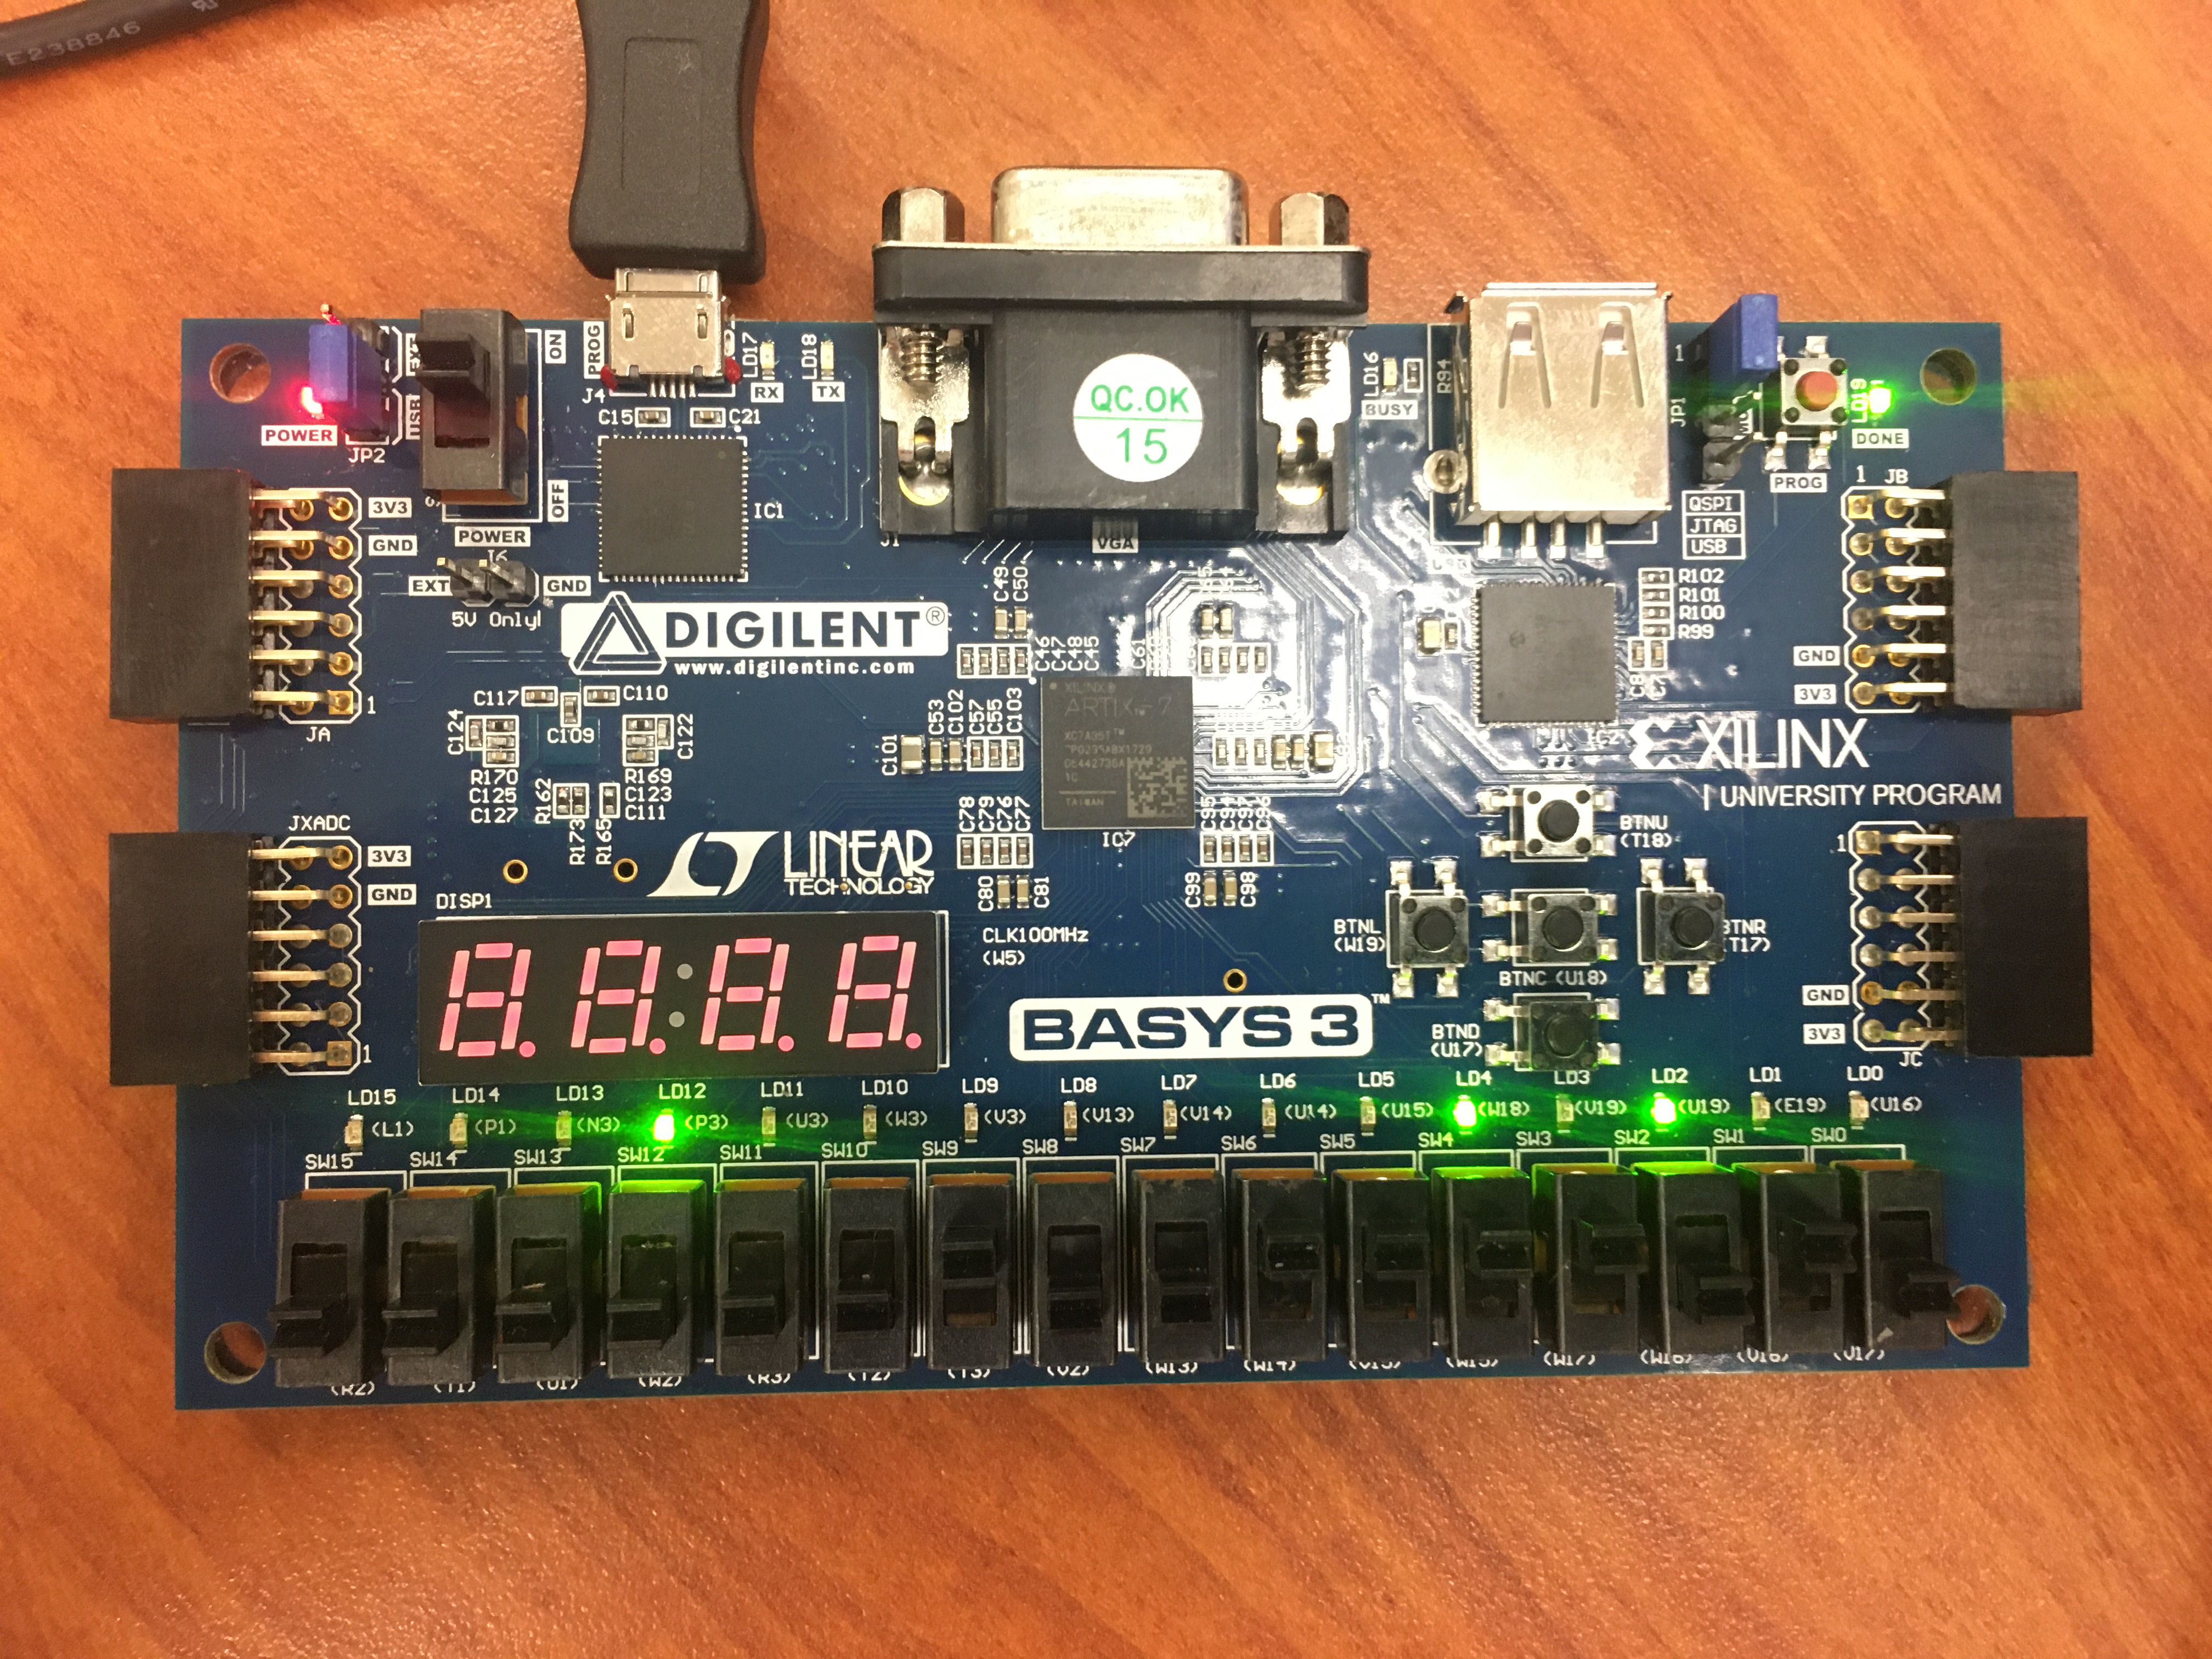
\includegraphics[width=12cm]{"board/and}
	\caption{AND Operation}
\end{figure}
\begin{figure}[ht]
	\centering
	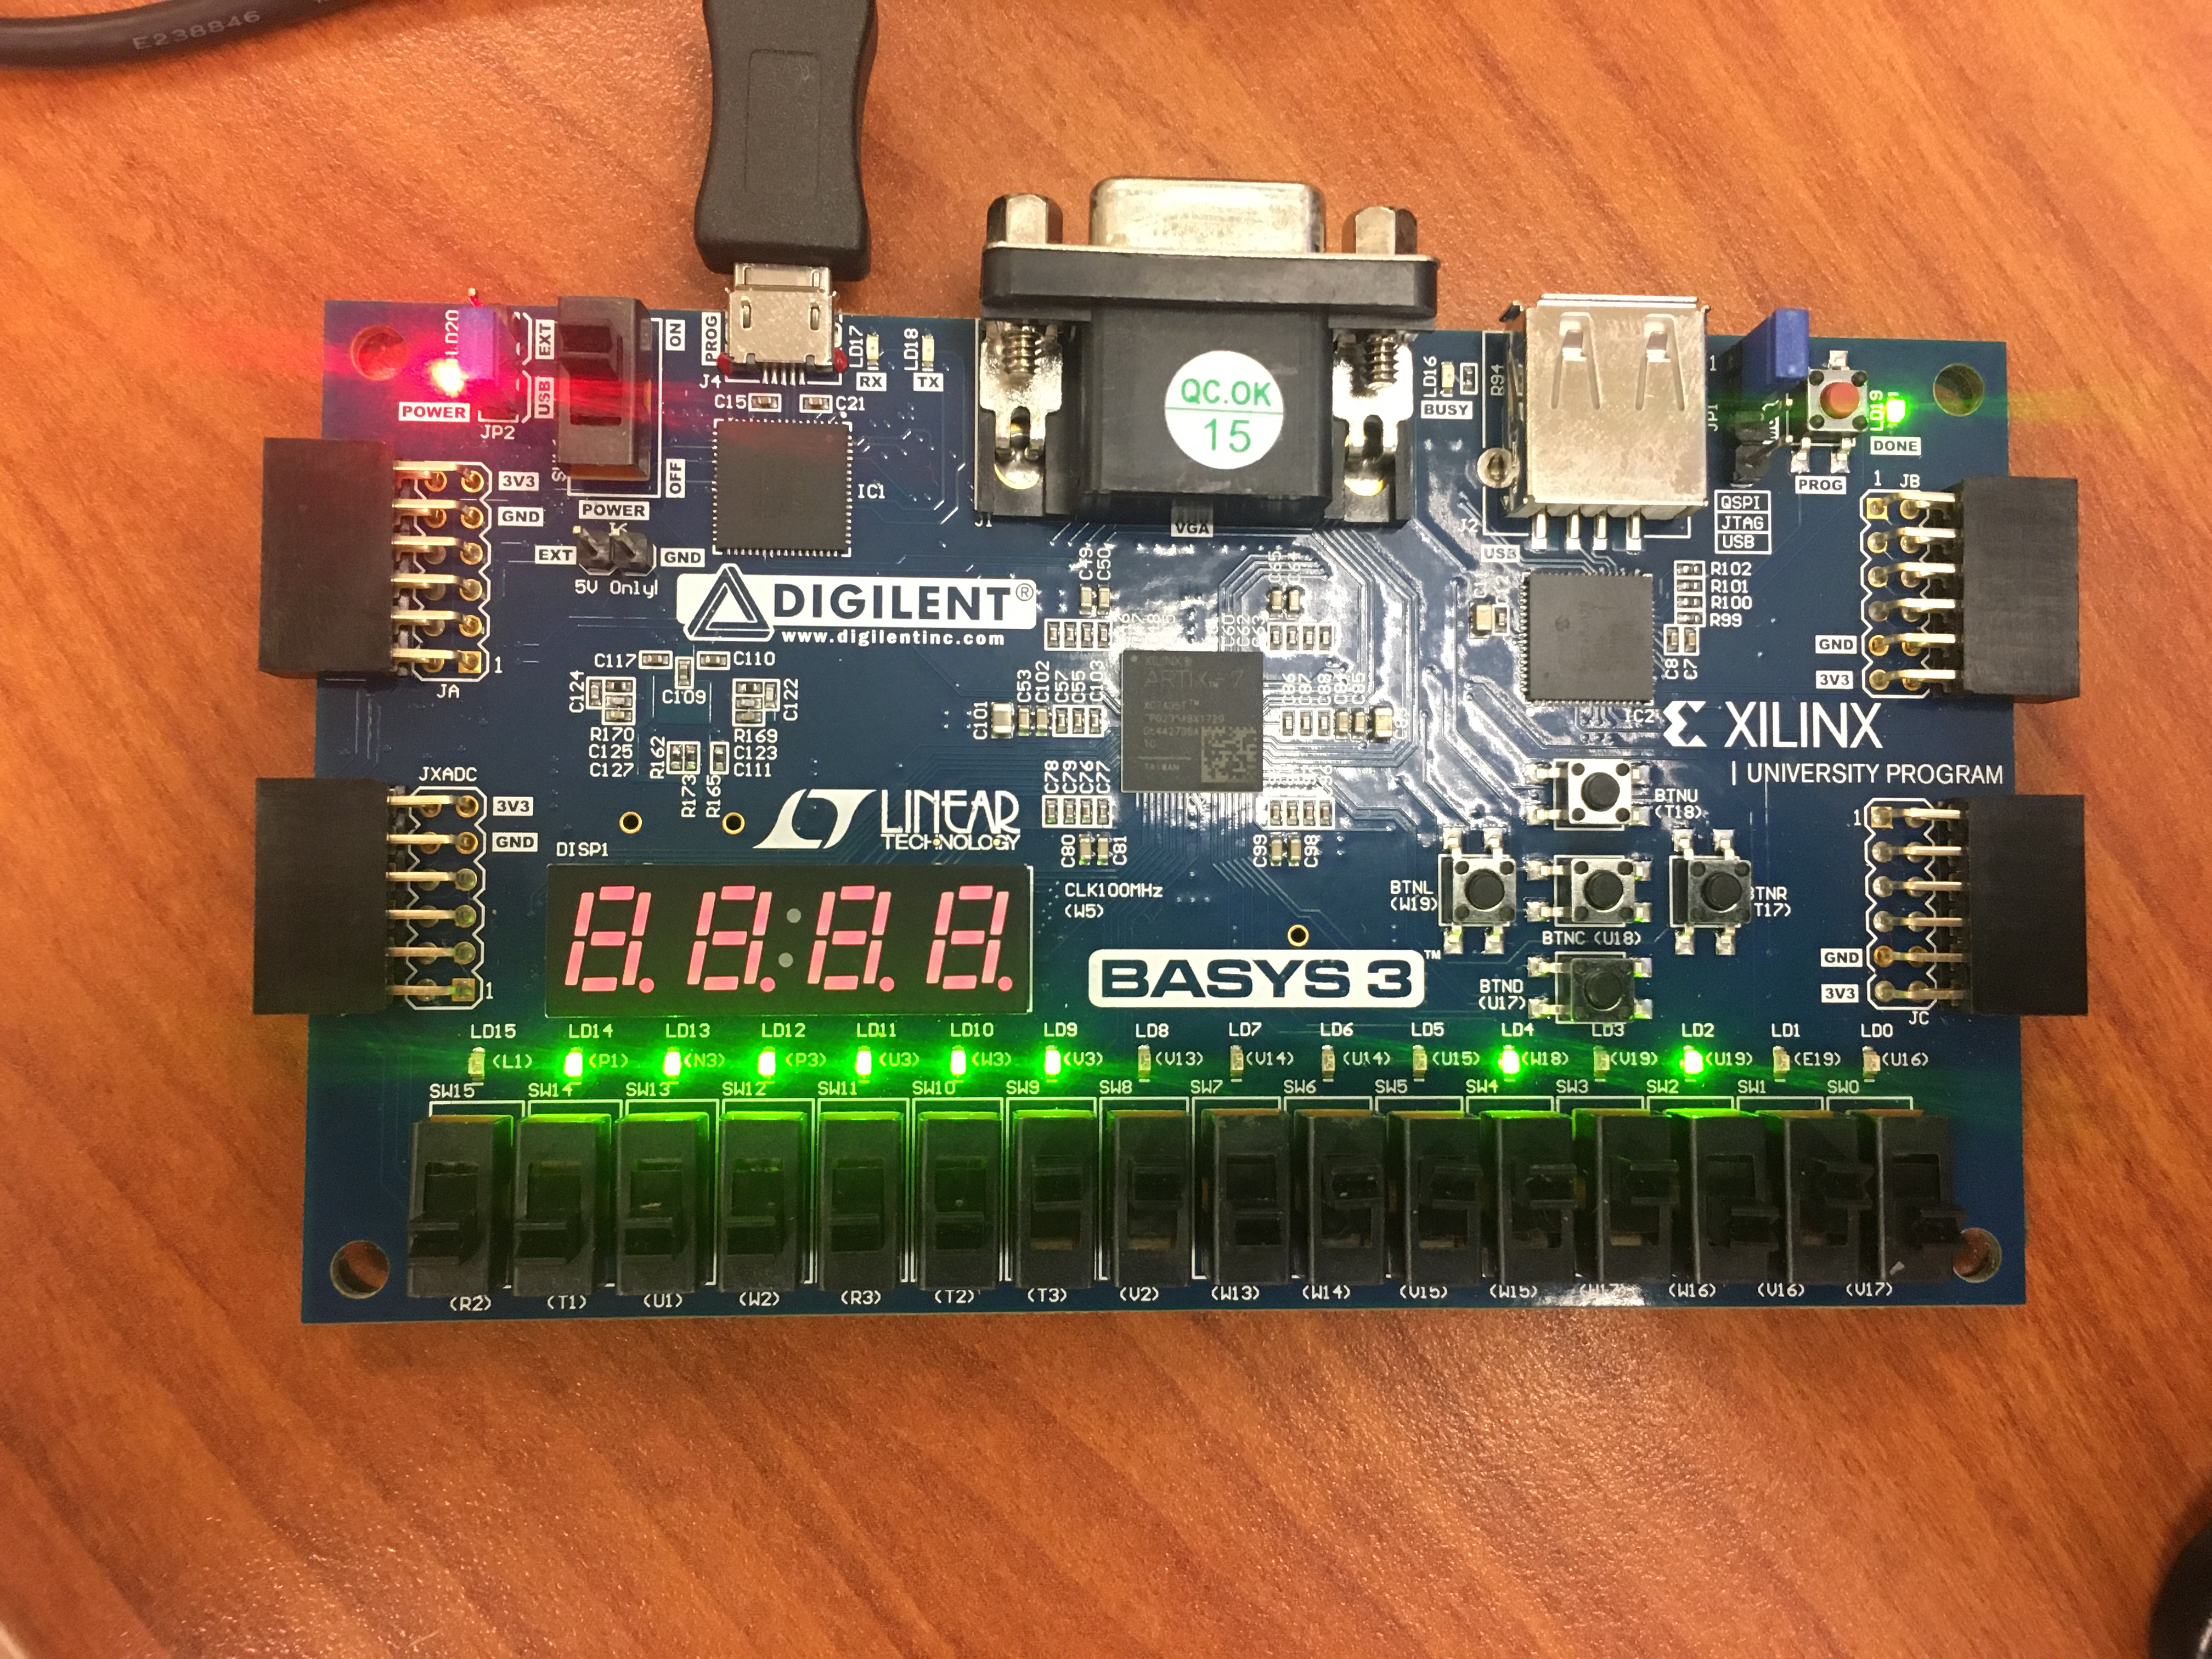
\includegraphics[width=12cm]{"board/or}
	\caption{OR Operation}
	\includegraphics[width=12cm]{"board/xor"}
	\caption{XOR Operation}
\end{figure}
\begin{figure}[ht]
	\centering
	\includegraphics[width=12cm]{"board/default"}
	\caption{Default Operation}
\end{figure}


\section*{Code}
\Verilog[firstline=23,caption=Register Implementation]{../verilog_code/register.sv}
\Verilog[firstline=23,caption=Register Test Bench]{../verilog_code/register_test.sv}
\Verilog[firstline=23,caption=ALU Implementation]{../verilog_code/alu.sv}
\Verilog[firstline=23,caption=ALU Test Bench]{../verilog_code/alu_test.sv}
\Verilog[firstline=23,caption=Top-Level Implementation]{../verilog_code/top_lab9.sv}

\end{document}
